\documentclass[tikz]{standalone}
\usepackage{pgfplots}
\pgfplotsset{compat=1.18}
\begin{document}
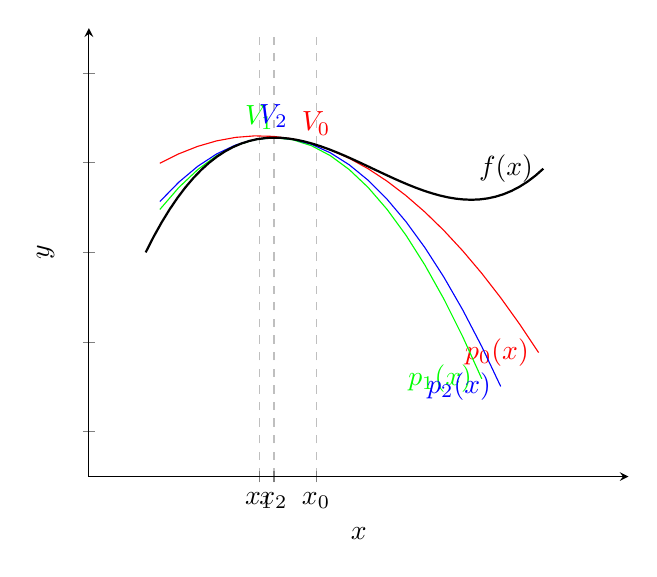
\begin{tikzpicture}
\begin{axis}[
    declare function={P(\x,\a,\b,\c)=\a*pow(\x,2)+\b*\x+\c;},
    axis lines=left,
    xlabel=$x$,
    ylabel=$y$,
    xmin=-7,xmax=2.5,
    ymin=-25,ymax=25,
    xtick={-4, -3.75, -3.732142857142857, -3},
    xticklabels={$x_1$, $x_2$, , $x_0$},
    yticklabels={},
    restrict x to domain=-6:1,
    restrict y to domain=-15:25,
    clip=false,
    xmajorgrids=true,
    grid style=dashed,
    %legend style={at={(axis cs:1,1)},anchor=nort west},
]
\xdef\xold{-3}
\xdef\yold{12}
\xdef\a{0}
\xdef\b{0}
\xdef\b{0}
%\pgfplotsforeachungrouped \k in {0,...,2}{
\foreach \k/\clr in {0/red,1/green,2/blue}{
    \pgfmathsetmacro{\a}{\xold + 2}
    \pgfmathsetmacro{\b}{1-pow(\xold, 2)}
    \pgfmathsetmacro{\c}{pow(\xold, 3) / 3 + 6}
    \pgfmathsetmacro{\xnew}{\xold - ((pow(\xold, 2) + 4*\xold + 1) / (2*\xold+4))}
    \pgfmathsetmacro{\ynew}{pow(\xnew,3)/3+2*pow(\xnew, 2)+\xnew+6}
    \edef\pt{\noexpand\addplot[
        only marks,
        mark=circle,
        mark size=3pt,
        point meta=explicit symbolic,
        nodes near coords,
        color=\clr
        ] coordinates {%
            (\xold,\yold) [$V_{\k}$]%
        };
    }
    \edef\px{\noexpand\addplot[
        domain=-5.75:2.25,
        color=\clr
        ]{P(x, \a, \b, \c)} node[left, pos=1]{$p_{\k}(x)$};
    }
    %\edef\ln{\noexpand\addplot[
    %    mark=none,
    %    color=\clr] coordinates {(\xold,\yold) (\xold,0)};
    %}
    \pt
    \px
    %\ln
    % variable update
    \global\let\xold\xnew
    \global\let\yold\ynew
}
\addplot[domain=-6:1,samples=51,color=black,thick]{x^3/3+2*x^2+x+6} node[left]{$f(x)$};
\end{axis}
\end{tikzpicture}
\end{document}

Informatica: Approssimazioni degli estremanti mediante vertici della parabola approssimante.

Matematica: Ricerca degli estremanti. Condizioni di esistenza di massimi e minimi. Punti stazionari.

Fisica: Energia potenziale ed equilibrio nei punti di minimo; configurazioni di minima energia; corrente elettrica (conduzione)

Scienze: orbitali, reazioni e bilanci energetici

Italiano: (da massimi e minimi alla bramosia del meglio) Il ciclo dei vinti, Verga

Storia: L'unità d'Italia (il periodo di ambientazione dei Malavoglia inizia nel 1861)

Filosofia: Il superuomo

Inglese: Un qualche autore di quel periodo storico
